\documentclass[13pt]{article}
\usepackage[hmargin=2cm, vmargin=3cm]{geometry}
\usepackage{mathtools}
\usepackage{amssymb}
\usepackage{amsthm}
\usepackage{enumerate}
\usepackage{graphicx}

\title{COMP 521 - Assignment 1}
\author{Yi Tian Xu\\260520039}
\date{Feburary 4, 2015}


\begin{document}
\maketitle
\section{Doorway/projectile behavior and interaction}

\subsection{Strategy for setting up the doors such that the maze is solvable}
The three sets of rooms are randomly chosen on a 30$\times$30 grid. One secondary room is picked to be connected with the exit. 

Then the braided maze is generated using Aldous-Broder/Wilson algorithm with the rest of the cells. When choosing a random branch to the maze, we allow the algorithm to choose a cell that it has already connected to the maze with a small probability except if the cell is part of a secondary room. This creates a braided maze with some doorway to the primary rooms.

To make sure that we have at least one doorway for each primary room, we randomly remove a wall from each primary room that is not part of a secondary room. Then we remove a wall between each primary room and its associated secondary room to make a door to the secondary room.

This allows the player to go to any primary room from the start of the maze. \\

The core functions for this part are in the file Maze.cs.

\subsection{Strategy for door/projectile and  anything-else/projectile interaction}
Each door from the primary room to the secondary room is set to a color that is the same as its corresponding projectile. A door only open when it's hit by a projectile of the same color. This is implemented as matching the tags of the colliding objects. 

In the game, the projectiles are design as large spheres. They are allowed to roll on the ground or bounce off the wall when they are projected. Thus to detect that a projectile did not hit its corresponding target, we check on the difference in its position between two frames. Once the difference hit a threshold, we assumes that it has come to a stop. This will notify another game object that will assume that this projectile did not hit its target unless or until its target comes notify that it got hit. If the target does not come to notify, then we can assume that the player has lose. 

\subsection{Player projectile interaction}
Player can pick up a projectile when that projectile is at most some small distance from the player. When we press ``.", we go through an array where the projectiles are store and check the distance. Once a projectile is used, it's removed from the array and thus can no longer be picked up. 

\subsection{Strategy for setting up the sequence of doorways the player need to take}
The order of the color is predetermined in the code. For the sake of notation, let $c_0$, $c_1$, $c_2$ and $c_4$ be the colors. The last projectile and the last doorway to the exit of the maze are always colored with $c_3$. 

Let $S_i$ be a secondary room with door color $c_i$, $i\in \{0,1,2\}$. Let $P_j$ be a projectile with color $c_j$, $j\in \{0,1,2,3\}$. 

Consider a randomly generated maze with a set of colored rooms and doors, a set of colored projectiles, an entrance and and the exit accessible from a secondary room $S_i$. $S_i$ must contain projectile $P_3$. Then our algorithm chooses:\\
$S_{[(i+1)\mod 3]}$ to contain projectile $P_i$;\\
$S_{[(i+2)\mod 3]}$ to contain projectile $P_{[(i+1)\mod 3]}$

Then we can set the entrance to contain projectile $P_{[(i+2)\mod 3]}$

This guarantees that the player must go through all the secondary room before exiting the maze. \\

This function is called \texttt{distributeBullets()} in file MazeManager.cs.

\section{Narrative}
Figure 1 shows the petri-net. 

The game is 1-pointless. When the player fires the projectiles while it's not aiming at the correct door, the player looses. But the player may not know that it looses until it goes near the used projectile, so that a text will display on the screen saying that the player is stuck in the maze forever. This takes one step.

As there is a path from any other state in the petri-net to the winning state, we have $p=1$.

\begin{figure}[ht!]
\center
 \caption{Petri-Net}
	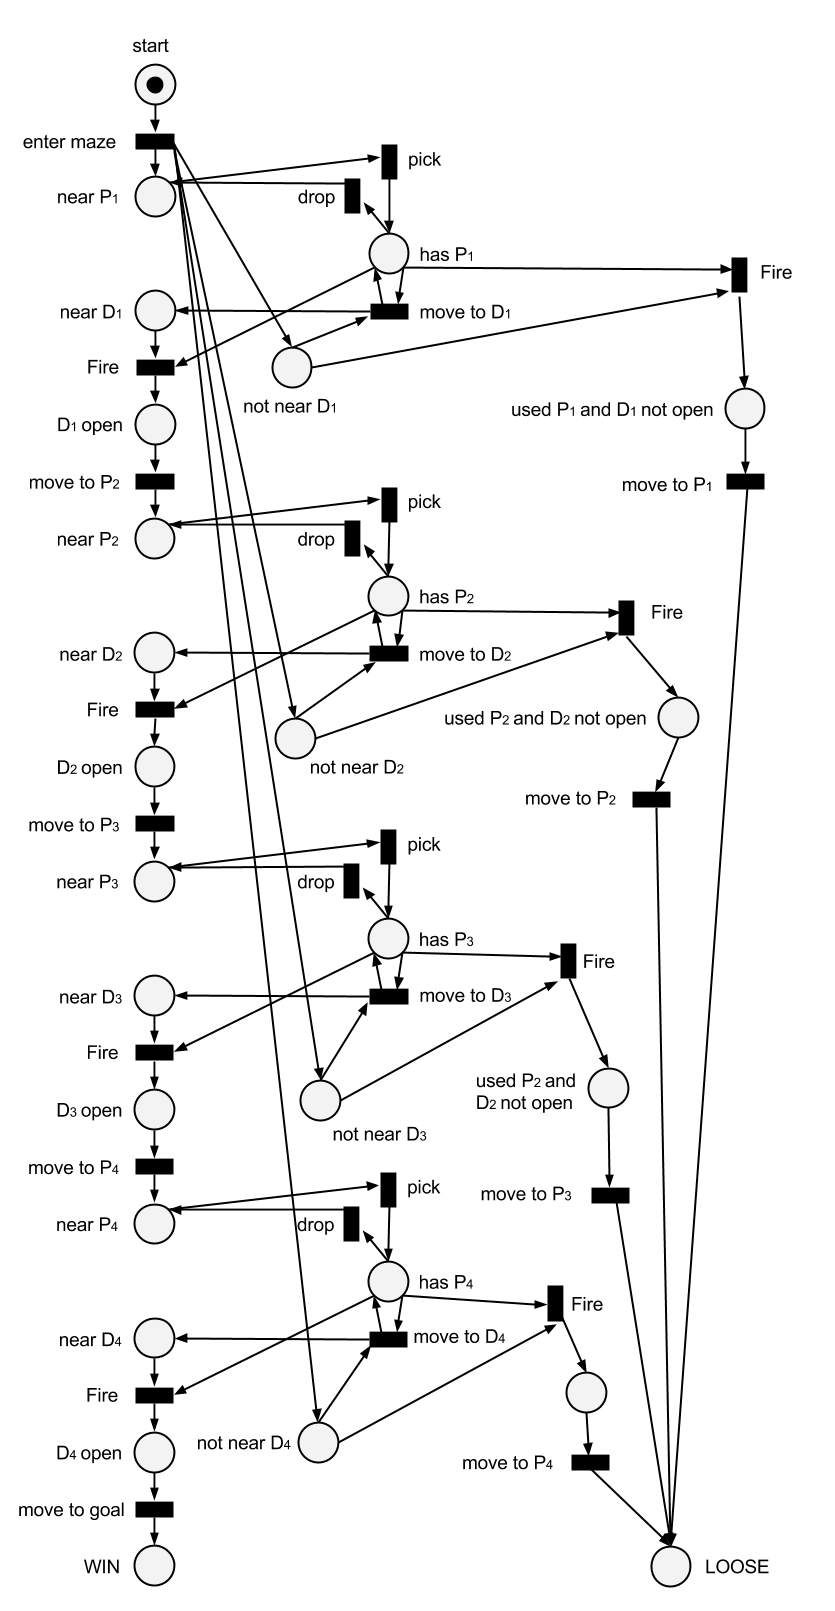
\includegraphics[width=115mm]{petri-net.png}
\end{figure}

\end{document}